\documentclass[12pt]{article}

\usepackage{amsmath,amssymb,amsthm}
\usepackage{geometry}
\usepackage{microtype}
\usepackage{hyperref}
\usepackage{tikz}
\usepackage{tikz-cd}
\usepackage{natbib}

\usetikzlibrary{
  arrows.meta,
  calc,
  positioning,
  decorations.pathmorphing,
  decorations.markings,
  fit,
  backgrounds
}

\geometry{margin=1.2in}

\newtheorem{definition}{Definition}
\newtheorem{proposition}{Proposition}
\newtheorem{theorem}{Theorem}
\newtheorem{remark}{Remark}

\title{Identity as Event History:\\
A Worked Introduction to Spherepop}
\author{Flyxion}
\date{\today}

\begin{document}

\maketitle

\begin{abstract}
Spherepop is a process-oriented formalism in which the identity of an object
is determined not by its present configuration but by the irreversible sequence
of transformations that produced it.  This essay develops the central principles
of the framework through a worked example and then situates those principles
within increasingly general mathematical structures: event words and normal
forms, directed acyclic event graphs, a categorical semantics of histories as
functors from causal index categories, a rewriting system for normalization, and
connections to trace theory, Petri nets, and string diagram formalisms.
Additional sections develop the order-theoretic structure of event histories as
posets and their linear extensions, a small-step operational semantics for
histories as labeled transition systems, measures of historical complexity
including depth and width, the historical reconstruction problem and its
relationship to informational irreversibility, a comparison of historical and
structural identity criteria, a treatment of Spherepop as a free traced monoidal
construction, and the connection to provenance graphs and distributed event logs.
Throughout, irreversibility is treated as the fundamental feature that gives
event histories their directed, acyclic character and that grounds a coherent
alternative to set-membership-based ontology.
\end{abstract}

\tableofcontents

\newpage

\section{Introduction}
\label{sec:introduction}

A recurring question in the foundations of mathematics and formal ontology
concerns the correct criterion of identity for objects that exist within
processes rather than in isolation.  Classical set theory locates identity in
the membership relation: two sets are equal precisely when they contain exactly
the same elements, irrespective of how those sets came to exist or in what order
their elements were assembled.  This extensional criterion is powerful and
convenient, but it discards what may be the most significant feature of many
objects encountered in physics, computation, and the theory of complex systems:
namely, that an object's identity is inseparable from the history that generated
it.

Spherepop is a formalism developed to address this gap directly.  Its central
claim is that objects should be represented not as static containers but as
\emph{records of transformations}, and that identity should be adjudicated by
comparing those records rather than by comparing present states.  The formalism
takes irreversibility as its organising principle.  Because the transformations
that produce objects cannot in general be undone, the historical record
accumulates monotonically; each new event appends to a trace that cannot be
retracted.  Two objects are therefore identical in the Spherepop sense if and
only if they are the products of identical histories.

This orientation connects Spherepop to a broad family of process-based theories.
In category theory, the importance of morphisms over objects is a foundational
methodological commitment \citep{MacLane1998}; histories composed of
irreversible events are naturally interpreted as compositions of morphisms, and
the event histories of objects become diagrams in causal categories.  In
theoretical computer science, the notion that computational identity should be
grounded in execution traces rather than in present memory states appears
implicitly throughout operational semantics \citep{Abramsky1994}.  In
concurrency theory, Mazurkiewicz traces \citep{Mazurkiewicz1987} provide an
established formalism for treating event sequences as equivalence classes
modulo independent commutation, and Spherepop event words can be understood as
canonical representatives of such classes.  In the theory of concurrent
processes, Petri nets \citep{Petri1966} provide a complementary operational
picture.

The present essay proceeds through several layers of increasing abstraction.
Section~\ref{sec:worked} presents the primary worked example, introducing two
processes that produce structurally similar objects by distinct histories and
establishing the foundational identity criterion.
Section~\ref{sec:eventwords} formalises this criterion through the notions of
event words and normal forms.  Section~\ref{sec:categorical} develops the
categorical interpretation, treating events as morphisms and histories as
compositions.  Section~\ref{sec:entropy} examines the relationship between
irreversibility and entropy.  Section~\ref{sec:dags} develops the directed
acyclic graph representation of event histories.
Section~\ref{sec:normalization} introduces normalization and canonical
representations.  Section~\ref{sec:functors} provides the functorial
perspective.  Section~\ref{sec:pushouts} examines merge events as pushout-like
constructions.  Section~\ref{sec:landscape} interprets histories as trajectories
across an entropy landscape.  Section~\ref{sec:posets} develops the partial-order
structure of event histories, establishing that event words are linear extensions
of the causal precedence relation.  Section~\ref{sec:complexity} introduces
quantitative measures of historical complexity including depth, width, and
branching factor.  Section~\ref{sec:operational} provides a small-step
operational semantics in which histories arise as execution traces of labeled
transition systems.  Section~\ref{sec:reconstruction} examines the historical
reconstruction problem and its relationship to informational irreversibility.
Section~\ref{sec:identity} compares the Spherepop historical identity criterion
with the extensional criterion of classical set theory.
Section~\ref{sec:equivalences} develops a stratified family of weaker
equivalence relations on histories.
Section~\ref{sec:traced} situates the framework within the theory of free
traced monoidal categories.
Section~\ref{sec:provenance} connects Spherepop to provenance graphs,
distributed event logs, and blockchain-style ledgers.
Appendices treat the BNF grammar for Spherepop expressions, the rewriting
system for normalization, the relationship to trace theory, Petri nets, and
string diagrams, and derived causal categories.


\section{A Worked Example}
\label{sec:worked}

To make the core principle concrete, consider an initial region $R$ and a
sequence of three events.  The first event, $E_1$, causes $R$ to split into
two descendant regions $A$ and $B$.  The second event, $E_2$, is a
transformation internal to $A$ that produces a new region $C$.  The third
event, $E_3$, causes the regions $B$ and $C$ to merge, producing the region
$D$.  Although the informal description is clear, the formal representation
of this history must record not merely which events occurred but in which
order they occurred and from which states each event proceeded.

Using the normal-form notation to be fully developed in
Section~\ref{sec:eventwords}, the history of each region is recorded as
follows.  Both $A$ and $B$ arose directly from $R$ through the single event
$E_1$, so their normal forms are identical:
\[
  (\text{spherepop}(A)) = (E_1), \qquad (\text{spherepop}(B)) = (E_1).
\]
The region $C$, however, arose from $A$ through the subsequent event $E_2$,
so its history includes both events:
\[
  (\text{spherepop}(C)) = (E_1, E_2).
\]
Finally, $D$ arose through the merger of $B$ and $C$, which itself required
all three events in order, so:
\[
  (\text{spherepop}(D)) = (E_1, E_2, E_3).
\]

The identity of each object is thus entirely determined by the ordered
sequence of events that produced it.  This is already a departure from
structural or compositional criteria: a criterion based on present structure
would describe $D$ solely in terms of what $D$ currently contains, with no
record of whether $D$ arose from a merger of previously split regions or from
some entirely different sequence of transformations.

To make this distinction sharp, consider a second process.  Suppose again
that $E_1$ causes $R$ to split into $A$ and $B$, but now suppose that instead
of $E_2$ there occurs a different event $E_3'$ that directly merges $A$ and
$B$ into a region $D'$, without the intermediate transformation that in the
first process generated $C$.  The normal form of $D'$ is then:
\[
  (\text{spherepop}(D')) = (E_1, E_3').
\]
Comparing the normal forms of $D$ and $D'$,
\[
  (\text{spherepop}(D)) = (E_1, E_2, E_3), \qquad
  (\text{spherepop}(D')) = (E_1, E_3'),
\]
the two histories are evidently distinct: $D$ accumulated three events while
$D'$ accumulated only two, and the events themselves differ.  The Spherepop
identity criterion therefore concludes that $D$ and $D'$ are not identical
objects, even if their present structural descriptions happen to agree.

This is the core claim of the formalism.  Structural indistinguishability is
insufficient for identity.  Two objects are identical in Spherepop precisely
when their complete generative histories, recorded in normal form, are
identical.


\section{Event Words and Normal Forms}
\label{sec:eventwords}

The worked example of Section~\ref{sec:worked} illustrates the central
representational idea intuitively.  To deploy it rigorously, the notion of a
history must be formalized as a structured symbolic object.

Let $\mathcal{E}$ denote the set of possible events in a given system.  Each
event in $\mathcal{E}$ corresponds to an irreversible transformation that
either produces new regions, modifies existing ones, or both.  The precise
physical or computational content of these events may vary; what matters for
the formalism is that they are discrete, ordered, and irreversible.

\begin{definition}[Event word]
An \emph{event word} over $\mathcal{E}$ is a finite ordered sequence
\[
  w = (E_{i_1}, E_{i_2}, \dots, E_{i_k})
\]
where each $E_{i_j} \in \mathcal{E}$.  The length of $w$ is $|w| = k$.  The
empty event word, denoting an object with no generative history, is written
$\varepsilon$.
\end{definition}

Because the events constituting a word are ordered, the same multiset of
events occurring in different sequences represents a different history.  This
ordering is not arbitrary: it encodes the causal and temporal precedence
relations among the events, about which more will be said when branching
histories are considered.

\begin{definition}[Spherepop normal form]
Spherepop associates to every object $X$ a canonical expression, the
\emph{normal form} of $X$, written $(\text{spherepop}(X))$, which is defined
to be the event word representing the complete generative history of $X$:
\[
  (\text{spherepop}(X)) = (E_{i_1}, E_{i_2}, \dots, E_{i_k}).
\]
\end{definition}

The normal form is the primary identity criterion of the formalism.  Two
objects are identical if and only if their normal forms coincide:
\[
  X \equiv Y
  \quad\Longleftrightarrow\quad
  (\text{spherepop}(X)) = (\text{spherepop}(Y)).
\]
This principle replaces identity criteria grounded in structural or
compositional properties.  Objects that are structurally indistinguishable
may nevertheless be distinct if their histories differ, and objects that
arose through entirely different structural pathways may be identical if
those pathways produced identical event sequences.

It is useful to visualize this criterion geometrically.  Figure~\ref{fig:trace}
represents an event word as a directed trace along a time axis, with the
irreversible events $E_1$, $E_2$, $E_3$ appearing as marked transitions
separating successive phases of the history.  The tick marks crossing the
trace axis emphasize that each transition is a genuine discontinuity: no
reversion to a prior state is possible.  The brace beneath the axis
indicates that the normal form $(\mathrm{spherepop}(D))_{\mathrm{nf}} =
(E_1, E_2, E_3)$ records the complete ordered content of that trace.

\begin{figure}[ht]
\centering
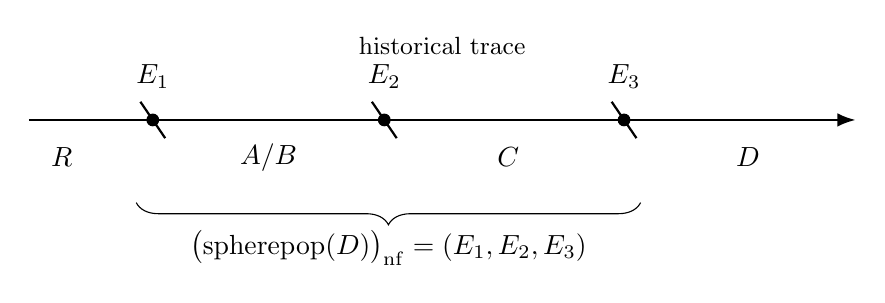
\begin{tikzpicture}[scale=1.05,>=Latex]
  \draw[thick,->] (0,0) -- (10,0);
  \filldraw (1.5,0) circle (2pt) node[above=8pt] {$E_1$};
  \filldraw (4.3,0) circle (2pt) node[above=8pt] {$E_2$};
  \filldraw (7.2,0) circle (2pt) node[above=8pt] {$E_3$};
  \node at (0.4,-0.45) {$R$};
  \node at (2.9,-0.45) {$A/B$};
  \node at (5.8,-0.45) {$C$};
  \node at (8.7,-0.45) {$D$};
  \foreach \x in {1.5,4.3,7.2} {
    \draw[thick] (\x-0.15,0.22) -- (\x+0.15,-0.22);
  }
  \draw[decorate,decoration={brace,mirror,amplitude=8pt}]
    (1.3,-1.0) -- (7.4,-1.0);
  \node at (4.35,-1.55)
    {$\bigl(\mathrm{spherepop}(D)\bigr)_{\mathrm{nf}}=(E_1,E_2,E_3)$};
  \node at (5,0.9) {\small historical trace};
\end{tikzpicture}
\caption{A geometric representation of an event word as an irreversible trace.
Tick marks indicate irreversible transitions; the brace records the
corresponding normal form.}
\label{fig:trace}
\end{figure}

The geometric picture reinforces a fundamental intuition: an object's position
on this trace cannot be recovered by inspecting the object alone.  Just as a
physical process that has dissipated energy cannot be run backwards to recover
the initial configuration, a Spherepop object does not carry within itself the
information necessary to reconstruct its generating history.  The normal form
is an external record, not an intrinsic property.

This historical criterion avoids several classical difficulties of set-based
ontology.  Objects in Spherepop are not defined by membership in collections
but by the irreversible sequences that produced them.  The ontology is
therefore inherently process-based: objects are histories rather than
containers, and the content of an object is its temporal structure rather than
its spatial extension.


\section{A Categorical Interpretation of Spherepop Histories}
\label{sec:categorical}

The representation of objects as event words suggests an immediate connection
with category theory, where the primacy of morphisms over objects is a
foundational methodological principle \citep{MacLane1998}.  In the categorical
framework, processes rather than states are primary; objects emerge as the
sources and targets of transformations, and the composition of morphisms
encodes the sequential structure of processes.  This perspective aligns
precisely with the Spherepop principle that identity is grounded in generative
history.

Let $\mathcal{C}$ be a category whose objects represent regions or
configurations of a system and whose morphisms represent irreversible events.
An event
\[
  E : X \rightarrow Y
\]
corresponds to a transformation that produces the region $Y$ from the region
$X$.  If two events occur sequentially,
\[
  E_1 : X \rightarrow Y, \qquad E_2 : Y \rightarrow Z,
\]
their categorical composition
\[
  E_2 \circ E_1 : X \rightarrow Z
\]
represents the combined historical process producing $Z$ from $X$.  In this
formulation, the event word introduced in Section~\ref{sec:eventwords}
corresponds precisely to a composition of morphisms, and the normal form of
an object is the morphism that takes the initial state to the present one.

Branching and merging events, which are prominent features of the worked
example, correspond to familiar categorical constructions.  A split event
\[
  E_1 : R \rightarrow A \sqcup B
\]
resembles a coproduct-like branching in which a single region gives rise to
multiple descendants, while a merge event
\[
  E_3 : (B, C) \rightarrow D
\]
resembles a pushout-like construction in which two regions produced from a
common ancestor are combined into a new one \citep{MacLane1998, Spivak2014}.
The precise categorical status of these constructions is examined further in
Section~\ref{sec:pushouts}; for present purposes it suffices to note that
the full history of the worked example forms a diagram in $\mathcal{C}$ of
the shape illustrated in Figure~\ref{fig:categorical}.

\begin{figure}[ht]
\centering
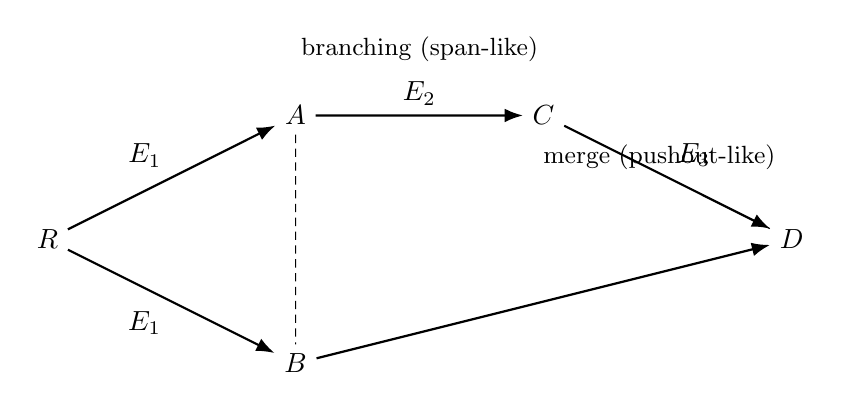
\begin{tikzpicture}[scale=1.05,>=Latex]
  \node (R) at (0,0)   {$R$};
  \node (A) at (3,1.5) {$A$};
  \node (B) at (3,-1.5){$B$};
  \node (C) at (6,1.5) {$C$};
  \node (D) at (9,0)   {$D$};
  \draw[thick,->] (R) -- node[above left]  {$E_1$} (A);
  \draw[thick,->] (R) -- node[below left]  {$E_1$} (B);
  \draw[thick,->] (A) -- node[above]       {$E_2$} (C);
  \draw[thick,->] (B) -- (D);
  \draw[thick,->] (C) -- node[above right] {$E_3$} (D);
  \draw[densely dashed] (A) -- (B);
  \draw[densely dashed] (C) -- (D);
  \node at (4.5,2.3)  {\small branching (span-like)};
  \node at (7.4,1.0)  {\small merge (pushout-like)};
\end{tikzpicture}
\caption{A categorical diagram of the worked example.  The split event $E_1$
produces a span, while the merge event $E_3$ completes a pushout-like
construction.  The identity of $D$ is determined by the entire diagram, not
merely by the node $D$ in isolation.}
\label{fig:categorical}
\end{figure}

From this perspective, the identity of an object is determined by the entire
diagram of morphisms that generated it.  Two objects are identical precisely
when the diagrams representing their histories are identical, up to equality of
morphisms.  This is a stronger condition than structural isomorphism of the
resulting objects; it requires agreement at every stage of the generative
process.

The categorical viewpoint also clarifies why Spherepop naturally produces
directed acyclic event graphs.  Cycles in a morphism-composition diagram would
correspond to reversible processes, since a path
\[
  X \rightarrow Y \rightarrow \dots \rightarrow X
\]
implies the existence of a composite morphism returning from $X$ to itself.  In
a setting where morphisms represent irreversible transformations, such a cycle
would violate the irreversibility condition.  The absence of cycles is therefore
not merely a convenient property but a structural consequence of the physical
or computational assumption that the events under consideration are
irreversible.  The relationship between irreversibility and directed acyclicity
is developed further in Section~\ref{sec:dags}, and the connection to entropy
is examined in Section~\ref{sec:entropy}.

\citet{BaezStay2010} describe in detail the deep correspondences among physics,
topology, logic, and computation through the ``Rosetta Stone'' of categorical
structures; the Spherepop framework sits naturally within the physical and
computational columns of that correspondence, where morphisms encode processes
and composition encodes sequential execution.


\section{Irreversibility and Entropy in Event Histories}
\label{sec:entropy}

The irreversibility of Spherepop events is not merely a formal stipulation; it
reflects a substantive claim about the physical and informational character of
the processes under consideration.  In thermodynamic systems, irreversible
transformations correspond to processes in which entropy increases and in which
information about prior states becomes dispersed across degrees of freedom that
are no longer practically accessible.  The connection between irreversibility
and entropy is therefore a natural one to explore within the Spherepop
framework, where each event appends a new term to a historical record that
cannot be retracted.

Consider again an event $E : X \rightarrow Y$ representing a transformation
that produces the region $Y$ from the region $X$.  In general, the inverse
transformation does not exist: one cannot recover $X$ uniquely from $Y$ alone.
Consequently the history of $Y$ cannot be reconstructed without additional
information beyond what $Y$ currently contains.  Spherepop responds to this
observation by treating the event history itself as the primary record, so
that the normal form
\[
  (\text{spherepop}(X)) = (E_{i_1}, E_{i_2}, \dots, E_{i_k})
\]
functions as a symbolic trace of the entropy-producing sequence of operations
that generated $X$.  Each event appends a new irreversible step to this trace,
and the trace cannot be shortened by any transformation available within the
system.

This motivates a natural measure of historical complexity.  If $H(X)$ denotes
the length of the event word associated with $X$,
\[
  H(X) = |(\text{spherepop}(X))|,
\]
then $H(X)$ provides a simple count of the irreversible operations that
separates $X$ from its initial state.  Each additional event increases the
informational content required to specify the object's origin.

More sophisticated formulations may weight individual events by their
informational or thermodynamic significance.  Define a weight function
$w : \mathcal{E} \rightarrow \mathbb{R}_{\geq 0}$ assigning to each event $E$
a non-negative real number $w(E)$ measuring its entropy contribution.  The
weighted historical complexity of $X$ is then
\[
  S(X) = \sum_{j=1}^{k} w(E_{i_j}).
\]
When $w$ is chosen to reflect genuine thermodynamic quantities, $S(X)$
provides an estimate of the total entropy produced along the history of $X$.
In general, the choice of $w$ encodes assumptions about the relative
significance of different classes of events, and different physical or
computational models will motivate different choices.

The geometric interpretation of this measure is illustrated in
Figure~\ref{fig:entropy}.  As events accumulate, the historical trace widens:
the cross-sectional thickness of the trajectory at each stage reflects the
growing informational content required to describe the object's origin.
Critical events that significantly increase $S(X)$ correspond to points of
rapid widening, while low-entropy events produce only modest expansion.

\begin{figure}[ht]
\centering
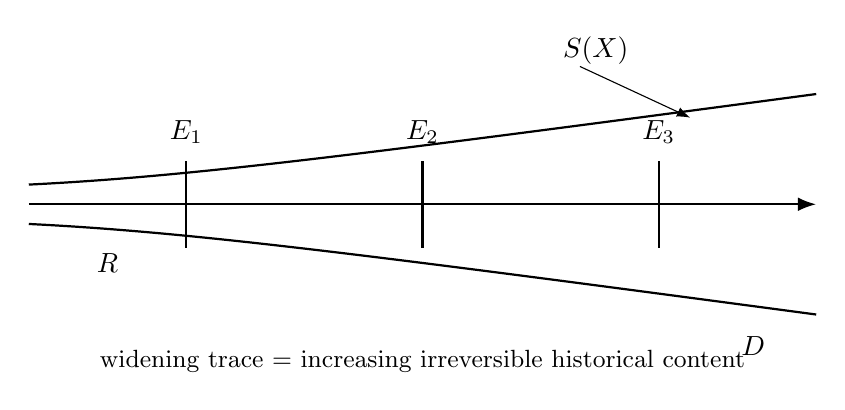
\begin{tikzpicture}[scale=1.0,>=Latex]
  \draw[thick,->] (0,0) -- (10,0);
  \draw[thick] (0,0.25)  .. controls (2,0.35)  and (4,0.6)  .. (10,1.4);
  \draw[thick] (0,-0.25) .. controls (2,-0.35) and (4,-0.6) .. (10,-1.4);
  \foreach \x/\lab in {2/E_1,5/E_2,8/E_3}{
    \draw[thick] (\x,-0.55) -- (\x,0.55);
    \node[above] at (\x,0.65) {$\lab$};
  }
  \node at (1,-0.75) {$R$};
  \node at (9.2,-1.8) {$D$};
  \node at (7.2,1.95) {$S(X)$};
  \draw[->] (7.0,1.75) -- (8.4,1.1);
  \node at (5,-2.0) {\small widening trace $=$ increasing irreversible historical content};
\end{tikzpicture}
\caption{Irreversible history represented as geometric widening.  As events
accumulate, the historical trace broadens, representing the growing
informational content that would be required to reconstruct the prior state.
The function $S(X)$ measures cumulative weighted entropy along the trace.}
\label{fig:entropy}
\end{figure}

This interpretation connects Spherepop to a broader class of process-based
theories in which the fundamental objects of a theory are not static states but
trajectories through configuration space.  In such theories, the informational
content of an object is the information required to specify its trajectory
rather than merely its present position.  The Spherepop normal form functions
as a compact symbolic encoding of this trajectory.

The resulting ontology is one in which entropy production provides the arrow of
time.  Because $S(X)$ is non-decreasing along any history---since all events
are assumed to contribute non-negatively to the weighted sum---histories are
naturally directed.  This directionality is not imposed externally as a formal
condition but emerges from the physical assumption that irreversible processes
increase entropy.  The directed acyclic structure of event histories, which is
treated as a formal property in the following section, therefore has a
thermodynamic grounding in the behaviour of $S(X)$ along any path through the
event graph.


\section{Event Graphs and Directed Acyclic Structure}
\label{sec:dags}

Linear event words provide a correct representation of histories in which each
event has at most one predecessor and at most one successor.  The processes
encountered in practice, however, frequently involve branching and merging: a
single region may give rise to multiple descendants, and multiple regions may
combine to produce a single new one.  In such cases the linear notation,
though applicable after a suitable ordering is imposed, obscures the parallel
structure of the history.  The natural representation is a directed graph.

\begin{definition}[Event graph]
An \emph{event graph} is a directed graph $G = (V, \mathcal{E})$ in which the
vertices $V$ represent regions and each directed edge $X \rightarrow Y$
represents an irreversible event producing the region $Y$ from the region $X$.
\end{definition}

When events produce multiple descendants or require multiple inputs, the
corresponding vertices in $G$ carry multiple outgoing or incoming edges
respectively.  The complete generative history of a system is encoded in the
global structure of $G$ rather than in any single path through it.

\begin{proposition}[Directed acyclicity]
Every Spherepop event graph is a directed acyclic graph (DAG).
\end{proposition}

\begin{proof}
Suppose for contradiction that $G$ contains a directed cycle
$X \rightarrow Y \rightarrow \cdots \rightarrow X$.  Then there exists a
composite event morphism that maps $X$ to itself, implying that the
transformation can be applied repeatedly to yield a reversible process
taking $X$ back to a state indistinguishable from $X$.  Since every
Spherepop event is irreversible by definition, such a composite cannot exist.
Consequently no directed cycle can occur in $G$.
\end{proof}

The directed acyclic property is not merely a convenience; it is the formal
analogue of the thermodynamic irreversibility condition formalized in
Section~\ref{sec:entropy}.  Every finite DAG admits a topological ordering, and
it is precisely this ordering that will be exploited by the normalization
procedure of Section~\ref{sec:normalization} to produce canonical event words
from branching histories.

Given an object $X$ appearing as a vertex in $G$, its identity is determined
not by the local properties of the vertex but by the global structure of the
subgraph that generated it.  Formally, let $\mathrm{Anc}(X)$ denote the set of
all vertices from which $X$ is reachable by a directed path in $G$.  The
\emph{ancestral subgraph} of $X$ is the induced subgraph
\[
  G_X = G[\mathrm{Anc}(X) \cup \{X\}]
\]
containing all vertices that contributed, directly or indirectly, to the
production of $X$.

\begin{definition}[Spherepop identity, graphical formulation]
Two objects $X$ and $Y$ are Spherepop-identical if and only if their
ancestral subgraphs $G_X$ and $G_Y$ are isomorphic as directed graphs with
edges labelled by event types.
\end{definition}

This definition subsumes the event-word formulation of Section~\ref{sec:eventwords}
as a special case: when histories are linear (no branching or merging), the
ancestral subgraph reduces to a directed path, and graph isomorphism reduces to
equality of the corresponding event sequences.

Figure~\ref{fig:dag} illustrates a more complex event graph containing multiple
levels of branching.  The terminal object $Z$ is determined by the entire
layered DAG structure feeding into it.  Different subsets of the graph
characterise different terminal objects; the identity criterion requires that
the complete ancestral subgraph, not merely the immediately preceding events,
be taken into account.

\begin{figure}[ht]
\centering
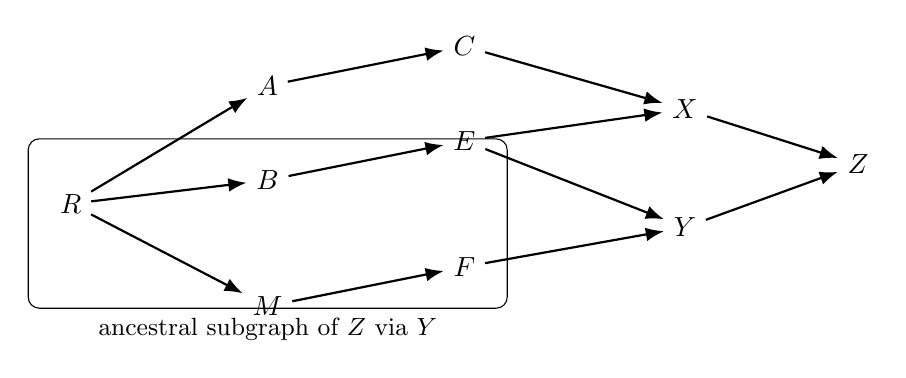
\begin{tikzpicture}[scale=1.0,>=Latex]
  \node (R) at (0,0)    {$R$};
  \node (A) at (2.5,1.5){$A$};
  \node (B) at (2.5,0.3){$B$};
  \node (M) at (2.5,-1.3){$M$};
  \node (C) at (5,2.0)  {$C$};
  \node (E) at (5,0.8)  {$E$};
  \node (F) at (5,-0.8) {$F$};
  \node (X) at (7.8,1.2){$X$};
  \node (Y) at (7.8,-0.3){$Y$};
  \node (Z) at (10,0.5) {$Z$};
  \foreach \u/\v in {R/A,R/B,R/M,A/C,B/E,M/F,C/X,E/X,E/Y,F/Y,X/Z,Y/Z}
    \draw[thick,->] (\u) -- (\v);
  \begin{scope}[on background layer]
    \node[draw,rounded corners,inner sep=8pt,
          fit=(R)(B)(F),
          label=below:{\small ancestral subgraph of $Z$ via $Y$}] {};
  \end{scope}
\end{tikzpicture}
\caption{A layered directed acyclic event graph.  The identity of the terminal
object $Z$ is determined by the entire ancestral subgraph that feeds into it,
not merely by its immediate predecessors $X$ and $Y$.}
\label{fig:dag}
\end{figure}

The DAG representation also clarifies the relationship between the event-word
notation and the diagrammatic structure.  A linear event word corresponds to a
directed path through the DAG.  Branching corresponds to a vertex with multiple
outgoing edges, and merging corresponds to a vertex with multiple incoming
edges.  The graph therefore provides a complete representation of the causal
structure, while the event word provides a linear serialization of that
structure.  The correspondence between these two representations is the subject
of the normalization theory in Section~\ref{sec:normalization}, where it is
shown that every event graph admits a canonical linear serialization.


\section{Normalization and Canonical Representation}
\label{sec:normalization}

The event graph representation captures the full causal structure of a history,
but different textual descriptions of the same graph may arise depending on
the order in which causally independent events are recorded.  If two events
act on disjoint regions without either depending on the output of the other,
then listing them in either order produces an equivalent description of the
same causal structure.  This equivalence must be recognized formally if the
identity criterion is to be stable under changes of representation.

\begin{definition}[Event independence]
Two events $E_i, E_j \in \mathcal{E}$ are \emph{independent}, written
$E_i \parallel E_j$, if neither event requires the output of the other as
input; equivalently, there is no directed path between $E_i$ and $E_j$ in the
event graph.
\end{definition}

Independent events may appear in either order in a linear serialization of the
event graph without altering the graph's structure.  This motivates the
following rewriting rule, which will be made precise in Appendix~\ref{app:rewriting}:

\[
  (E_i, E_j) \;\longrightarrow\; (E_j, E_i)
  \quad \text{whenever } E_i \parallel E_j.
\]

Two event words are \emph{causally equivalent} if they are related by a finite
sequence of such commutation steps.  The normalization procedure selects a
canonical representative from each causal equivalence class.

\begin{definition}[Spherepop normal form, canonical]
The \emph{Spherepop normal form} of an object $X$ is the event word
\[
  (\text{spherepop}(X))_{\mathrm{nf}}
\]
obtained by computing a topological ordering of the event graph $G_X$ and
serializing the events in that order, breaking ties consistently according to
a fixed deterministic convention on event labels.
\end{definition}

Because every finite DAG admits a topological ordering, and because the
normalization procedure is deterministic, the normal form is well-defined for
every Spherepop object.  The canonical identity condition becomes:
\[
  X \equiv Y
  \quad\Longleftrightarrow\quad
  (\text{spherepop}(X))_{\mathrm{nf}} = (\text{spherepop}(Y))_{\mathrm{nf}}.
\]

Two objects are identical exactly when their normalized event histories
coincide, regardless of the particular serialization that may have been used
to describe their histories in the first instance.

Figure~\ref{fig:normalization} illustrates this point concretely.  Two
syntactically different presentations of the same history---one listing $E_i$
before $E_j$ and the other listing $E_j$ before $E_i$ on two parallel
branches---both normalize to the same canonical form, because the two events
are independent and the topological ordering convention resolves the tie
deterministically.

\begin{figure}[ht]
\centering
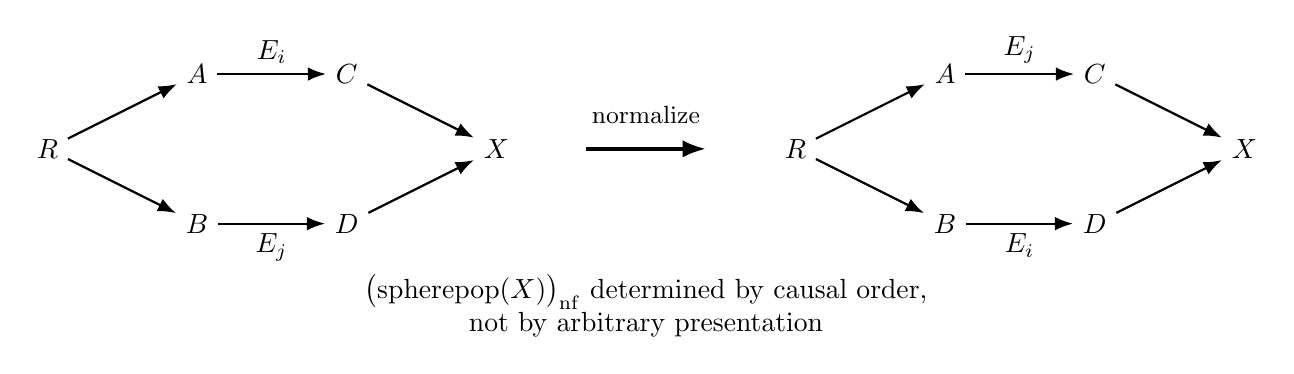
\begin{tikzpicture}[scale=0.95,>=Latex]
  \node (R1) at (0,0)   {$R$};
  \node (A1) at (2,1)   {$A$};
  \node (B1) at (2,-1)  {$B$};
  \node (C1) at (4,1)   {$C$};
  \node (D1) at (4,-1)  {$D$};
  \node (X1) at (6,0)   {$X$};
  \draw[thick,->] (R1)--(A1);
  \draw[thick,->] (R1)--(B1);
  \draw[thick,->] (A1)-- node[above] {$E_i$} (C1);
  \draw[thick,->] (B1)-- node[below] {$E_j$} (D1);
  \draw[thick,->] (C1)--(X1);
  \draw[thick,->] (D1)--(X1);
  \node (R2) at (10,0)  {$R$};
  \node (A2) at (12,1)  {$A$};
  \node (B2) at (12,-1) {$B$};
  \node (C2) at (14,1)  {$C$};
  \node (D2) at (14,-1) {$D$};
  \node (X2) at (16,0)  {$X$};
  \draw[thick,->] (R2)--(A2);
  \draw[thick,->] (R2)--(B2);
  \draw[thick,->] (A2)-- node[above] {$E_j$} (C2);
  \draw[thick,->] (B2)-- node[below] {$E_i$} (D2);
  \draw[thick,->] (C2)--(X2);
  \draw[thick,->] (D2)--(X2);
  \draw[very thick,->] (7.2,0) -- (8.8,0);
  \node at (8,0.45) {\small normalize};
  \node[align=center] at (8,-2.1)
    {$\bigl(\mathrm{spherepop}(X)\bigr)_{\mathrm{nf}}$
     determined by causal order,\\not by arbitrary presentation};
\end{tikzpicture}
\caption{Two syntactically different presentations of independent events $E_i$
and $E_j$ encoding the same causal structure.  Normalization collapses both to
a single canonical form, since $E_i \parallel E_j$ implies their order may be
resolved by any fixed topological convention.}
\label{fig:normalization}
\end{figure}

The normalization procedure plays a role in Spherepop analogous to that of
canonical forms in other mathematical frameworks: reduced words in group theory,
row echelon form in linear algebra, beta-normal forms in the lambda calculus.
Each of these devices converts a syntactically diverse family of equivalent
expressions into a unique representative that can be compared directly.  In
Spherepop, the canonical form ensures that identity depends only on causal
structure rather than on the order in which an external observer happened to
record causally independent events.


\section{Functorial Perspectives on Event Histories}
\label{sec:functors}

The event graph representation and the normalization theory of
Section~\ref{sec:normalization} can be cast in a fully categorical language by
treating the process of mapping abstract causal structures onto concrete systems
as a functor.  This perspective, which draws on the categorical foundations
developed in \citet{MacLane1998} and elaborated in \citet{Spivak2014} and
\citet{BaezStay2010}, provides the most general formulation of Spherepop
semantics.

\begin{definition}[Causal history category]
Let $\mathcal{H}$ be a small category whose objects represent intermediate
regions or states in a history and whose morphisms represent irreversible
events.  Because the events are temporally ordered and irreversible, if there
exists a morphism $X \rightarrow Y$ in $\mathcal{H}$ then there cannot exist
a morphism $Y \rightarrow X$.  Such a category is called a \emph{causal
history category}.
\end{definition}

In practice, $\mathcal{H}$ may be constructed directly from the event graph
$G$ by interpreting vertices as objects and directed edges as generating
morphisms, with composition given by directed paths.  The temporal ordering
that the DAG structure imposes on $G$ corresponds to the ``no-back-morphism''
condition in $\mathcal{H}$.

\begin{definition}[Spherepop realization functor]
Let $\mathcal{C}$ be a category of regions, configurations, or system states.
A \emph{Spherepop realization} of the history $\mathcal{H}$ in $\mathcal{C}$
is a functor
\[
  F : \mathcal{H} \rightarrow \mathcal{C}.
\]
\end{definition}

The functor $F$ assigns to each node in the abstract causal history a concrete
object in $\mathcal{C}$, and to each event morphism the corresponding
transformation in the physical or computational system.  Functoriality ensures
that sequential composition of events in $\mathcal{H}$ corresponds exactly to
sequential composition of transformations in $\mathcal{C}$:
\[
  F(E_2 \circ E_1) = F(E_2) \circ F(E_1).
\]
This coherence condition is the categorical expression of the physical
requirement that the combined effect of two sequential events is the
composition of their individual effects, without hidden intermediate states.

Terminal objects of $\mathcal{H}$ correspond to the currently existing objects
of the system---those that have not been further transformed.  If $X$ is such a
terminal node, then $F(X)$ represents the concrete present state produced by
the entire chain of events that preceded it.  The identity of $F(X)$ as a
Spherepop object is determined jointly by $F$ and by the position of $X$ in
the causal diagram.

Figure~\ref{fig:functor} illustrates the functorial picture.  The abstract
causal history category $\mathcal{H}$ on the left carries the relational
structure of the history---which events preceded which---without specifying
their concrete content.  The functor $F$ maps this abstract structure into the
category $\mathcal{C}$ of realized regions on the right, where each abstract
node becomes a concrete object and each abstract morphism becomes a concrete
transformation.

\begin{figure}[ht]
\centering
\begin{tikzpicture}[scale=1.0,>=Latex]
  \node (hR) at (0,0)    {$r$};
  \node (hA) at (2,1.2)  {$a$};
  \node (hB) at (2,-1.2) {$b$};
  \node (hD) at (4,0)    {$d$};
  \draw[thick,->] (hR) -- (hA);
  \draw[thick,->] (hR) -- (hB);
  \draw[thick,->] (hA) -- (hD);
  \draw[thick,->] (hB) -- (hD);
  \node at (2,-2.0) {$\mathcal{H}$};
  \draw[very thick,->] (5.2,0) -- (8.3,0);
  \node at (6.7,0.45) {$F$};
  \node (cR) at (10,0)   [circle,draw,inner sep=1.5pt] {};
  \node (cA) at (12,1.4) [circle,draw,inner sep=1.5pt] {};
  \node (cB) at (12,-1.4)[circle,draw,inner sep=1.5pt] {};
  \node (cD) at (14,0)   [circle,draw,inner sep=1.5pt] {};
  \draw[thick,->] (cR) -- (cA);
  \draw[thick,->] (cR) -- (cB);
  \draw[thick,->] (cA) -- (cD);
  \draw[thick,->] (cB) -- (cD);
  \draw[densely dashed] (9.5,-0.5) ellipse (0.8 and 0.5);
  \draw[densely dashed] (12,1.4)   ellipse (0.9 and 0.55);
  \draw[densely dashed] (12,-1.4)  ellipse (0.9 and 0.55);
  \draw[densely dashed] (14,0)     ellipse (1.1 and 0.75);
  \node at (12,-2.0) {$\mathcal{C}$};
\end{tikzpicture}
\caption{A Spherepop history as a functor $F : \mathcal{H} \rightarrow \mathcal{C}$
from an abstract causal index category $\mathcal{H}$ to a category $\mathcal{C}$
of realized regions.  The abstract structure on the left encodes causal
precedence; the functor translates this into concrete transformations on the right.}
\label{fig:functor}
\end{figure}

The functorial formulation also provides a clean account of when two objects
should be considered identical.  Suppose
\[
  F_1 : \mathcal{H}_1 \rightarrow \mathcal{C}
  \quad\text{and}\quad
  F_2 : \mathcal{H}_2 \rightarrow \mathcal{C}
\]
are two realizations.  The resulting terminal objects coincide as Spherepop
objects when the normalized causal structures $\mathcal{H}_1$ and $\mathcal{H}_2$
are isomorphic as causal categories and the functors agree on the corresponding
morphisms under this isomorphism.  This condition recovers the normal-form
identity criterion of Section~\ref{sec:normalization} in categorical language:
it requires agreement not merely on terminal values but on the entire
structure of the generating process.

The functorial perspective also suggests how Spherepop should handle
abstraction.  Natural transformations between realizations---that is, morphisms
in the functor category $[\mathcal{H}, \mathcal{C}]$---correspond to
systematic reinterpretations of a history that change the concrete objects
assigned to nodes while preserving the relational structure.  In this way the
framework supports a hierarchy of increasingly abstract descriptions of the
same underlying causal history.


\section{Merge Events as Pushouts}
\label{sec:pushouts}

The merge events that appear prominently in Spherepop histories admit a precise
categorical characterization as pushout constructions.  A pushout in a category
$\mathcal{C}$ is the universal solution to the problem of combining two
morphisms that share a common source: given morphisms $f : R \rightarrow B$ and
$g : R \rightarrow C$, the pushout is an object $D$ together with morphisms
$B \rightarrow D$ and $C \rightarrow D$ such that the resulting square commutes
and $D$ is universal with this property \citep{MacLane1998}.

The connection to Spherepop is direct.  In the worked example of
Section~\ref{sec:worked}, the regions $B$ and $C$ both originated from the
common ancestor $R$ via the split event $E_1$.  The merge event $E_3$ then
combined $B$ and $C$ into the region $D$.  Categorically, this situation is
described by the commuting square
\[
\begin{tikzcd}
  R \arrow[r] \arrow[d] & C \arrow[d] \\
  B \arrow[r]           & D
\end{tikzcd}
\]
in which $D$ receives consistent morphisms from $B$ and $C$ and is universal
with this property.  The merge event $E_3$ corresponds precisely to the
completion of this pushout diagram.

\begin{figure}[ht]
\centering
\begin{tikzpicture}[scale=1.05,>=Latex]
  \node (R) at (0,0)  {$R$};
  \node (C) at (3,2)  {$C$};
  \node (B) at (3,-2) {$B$};
  \node (D) at (6,0)  {$D$};
  \draw[thick,->] (R) -- (C);
  \draw[thick,->] (R) -- (B);
  \draw[thick,->] (C) -- (D);
  \draw[thick,->] (B) -- (D);
  \node at (3,0) {$\square$};
\end{tikzpicture}
\caption{A merge event represented as a pushout-like square.  The common ancestor $R$
gives rise to $B$ and $C$ via the split event; the merge event $E_3$ completes
the square by producing the universal object $D$.}
\label{fig:pushout}
\end{figure}

The pushout interpretation makes precise the sense in which the identity of
$D$ depends on the entire commuting square rather than merely on the pair
$(B, C)$ considered in isolation.  Two regions $B'$ and $C'$ could be merged
to produce a region $D'$ with the same structural description as $D$, yet if
$B'$ and $C'$ arose from a different common ancestor $R'$, the resulting
pushout square would be different and $D'$ would be a different Spherepop
object.  The pushout construction thus encodes the relational history of the
merge event, not merely its output.

This observation connects to the broader theme of the paper.  In standard
set-theoretic or structural accounts of identity, two sets are equal when they
contain the same elements, regardless of how those elements were assembled.
The pushout characterization of merge events shows that in Spherepop the
corresponding condition is far stronger: the merged object must have arisen
from the same causal configuration, with the same common ancestor and the same
morphisms connecting it to its predecessors.

The pushout interpretation also interacts with the categorical coherence
conditions noted in Section~\ref{sec:functors}.  A realization functor
$F : \mathcal{H} \rightarrow \mathcal{C}$ that preserves pushouts maps each
merge event in the abstract history to a genuine pushout in the target
category.  When $\mathcal{C}$ is a category with all pushouts---for instance,
a category of sets or a category of topological spaces---this preservation
condition is automatically satisfied.  In physical applications, the relevant
category may not have all pushouts, and the question of when merge events can
be faithfully realized is a substantive one.


\section{Entropy Landscapes and Historical Trajectories}
\label{sec:landscape}

A complementary geometric interpretation of Spherepop histories arises from
the notion of an entropy landscape.  This interpretation is more impressionistic
than the category-theoretic treatment of preceding sections, but it connects
the formalism to physical intuitions about the role of irreversibility in
shaping the space of possible histories.

Let the configuration space of a system be represented as a manifold
$\mathcal{M}$ whose points correspond to possible structural states.  Define an
entropy-like functional
\[
  S : \mathcal{M} \rightarrow \mathbb{R}
\]
measuring the informational or thermodynamic complexity of each state.
Irreversible events may then be interpreted as transitions that move the system
along trajectories in $\mathcal{M}$ while generally increasing the value of
$S$.  The history of an object corresponds to a directed path through this
landscape, constrained to move in the direction of increasing $S$.

\begin{figure}[ht]
\centering
\begin{tikzpicture}[scale=1.0]
  \draw[thick] (-4,0) .. controls (-2,2) and (-1,1) .. (0,3)
               .. controls (1,5) and (3,3) .. (4,4);
  \draw[thick] (-4,0) .. controls (-2,-2) and (-1,-1) .. (0,-3)
               .. controls (1,-5) and (3,-3) .. (4,-4);
  \draw[very thick,->] (-3,0) -- (-1.5,0.8);
  \draw[very thick,->] (-1.5,0.8) -- (0.2,2.2);
  \draw[very thick,->] (0.2,2.2) -- (2.2,3.6);
  \node at (-3.2,0.4) {$E_1$};
  \node at (-1.5,1.4) {$E_2$};
  \node at (0.9,3.0)  {$E_3$};
  \node at (3.2,4.6)  {$S$};
\end{tikzpicture}
\caption{Event history interpreted as a directed trajectory across an entropy
landscape.  Each event corresponds to a transition along a path that generally
moves toward regions of higher entropy.  The topology of the landscape
constrains which transitions are possible.}
\label{fig:landscape}
\end{figure}

In this geometric picture, as illustrated in Figure~\ref{fig:landscape}, the
events $E_1$, $E_2$, $E_3$ correspond to successive steps along a trajectory
that climbs the entropy surface.  The shape of the landscape determines which
transitions are available at each point: a configuration at a local minimum of
$S$ that is not a global minimum may be accessible from some prior states but
inaccessible from others, and the question of reachability depends on the
full path taken up to that point.  This path-dependence is precisely the
feature that Spherepop captures through its event-word representation: the
normal form records not just the endpoint of the trajectory but the entire
path.

Critical points of the entropy functional may be interpreted as stable
structural configurations or attractor states.  The Spherepop history of an
object records the sequence of transitions that led to its current position on
the landscape, including which saddle points and ridges it passed through on
the way.  Two objects at the same configuration on the landscape but arriving
via different paths are therefore different Spherepop objects, even though a
purely spatial description would identify them.

The entropy landscape interpretation also suggests a connection to the theory
of gradient flows and Morse theory, where the topology of a functional landscape
constrains the structure of trajectories and the classification of critical
points.  Spherepop histories can in principle be studied using these geometric
tools to understand, for instance, which pairs of histories are deformable into
one another through the insertion or deletion of null events, or how the
topology of the causal DAG interacts with the geometry of the underlying
landscape.  This direction of generalization lies beyond the scope of the
present essay but suggests a rich programme of further investigation.


\section{Event Histories as Partial Orders}
\label{sec:posets}

The directed acyclic structure of Spherepop event graphs implies that each
history carries a natural partial order on its events.  Making this structure
explicit provides a useful bridge between the graph-theoretic and algebraic
representations of histories developed in previous sections, and connects the
Spherepop framework directly to classical order theory and the concurrency-
theoretic tradition of Mazurkiewicz \citep{Mazurkiewicz1987}.

Let $G = (V, \mathcal{E})$ be an event graph.  Define a binary relation
$\prec$ on the set of events by declaring
\[
  E_i \prec E_j
\]
whenever there exists a directed path from $E_i$ to $E_j$ in $G$.  The
following proposition is immediate from the DAG property established in
Section~\ref{sec:dags}.

\begin{proposition}
The relation $\prec$ is a strict partial order on the set of events of any
Spherepop history.
\end{proposition}

\begin{proof}
Irreflexivity holds because the event graph is acyclic: no event can appear
on a directed path that begins and ends at itself.  Asymmetry is immediate from
the same acyclicity: if $E_i \prec E_j$ then there is a directed path from
$E_i$ to $E_j$, and the existence of a directed path from $E_j$ to $E_i$ would
close a cycle.  Transitivity follows by concatenating directed paths: if
$E_i \prec E_j$ and $E_j \prec E_k$ then the composed path witnesses
$E_i \prec E_k$.
\end{proof}

Each Spherepop history therefore determines a partially ordered set
$(\mathcal{E}_X, \prec)$, called the \emph{causal poset} of $X$.  The
incomparable elements of this poset are precisely the mutually independent
events: two events $E_i$ and $E_j$ satisfy $E_i \parallel E_j$ if and only if
neither $E_i \prec E_j$ nor $E_j \prec E_i$.

The event words introduced in Section~\ref{sec:eventwords} can now be
interpreted with precision as \emph{linear extensions} of the causal poset.

\begin{definition}[Linear extension]
A \emph{linear extension} of $(\mathcal{E}_X, \prec)$ is a total ordering
$\leq$ of $\mathcal{E}_X$ such that $E_i \prec E_j$ implies $E_i \leq E_j$.
\end{definition}

Every topological ordering of the event graph $G_X$ corresponds to a linear
extension of the causal poset, and conversely every linear extension arises
from some topological ordering.  The collection of all linear extensions
therefore coincides precisely with the set of all event words that are causally
equivalent in the sense of Section~\ref{sec:normalization}: they represent
different serializations of the same partial order.

This observation reframes normalization in order-theoretic terms.  The
commutation rules that identify independent events are precisely the moves
that relate different linear extensions of the same poset.  The Spherepop
normal form selects a canonical linear extension by fixing a deterministic
rule for breaking incomparability ties.

The width of the causal poset, which counts the size of the largest antichain,
measures the maximal degree of parallelism in the history.  Dilworth's theorem
\citep{MacLane1998} states that the minimum number of chains needed to partition
the poset equals the width; in the Spherepop context this means that the most
compressed sequential description of a history requires at least as many
serialized chains as the width of its causal poset.  Wide histories represent
highly parallel processes that cannot be faithfully compressed into a single
short sequential trace.

The partial-order perspective thus provides the algebraic underpinning for both
the normalization theory and the complexity measures developed in the next
section, tying these constructions to the classical theory of posets and their
linear extensions.


\section{Historical Complexity Measures}
\label{sec:complexity}

The entropy measure $S(X)$ introduced in Section~\ref{sec:entropy} captures
the cumulative informational weight of a history by summing the contributions
of individual events.  A complementary family of measures can be derived
directly from the structure of the causal poset $(\mathcal{E}_X, \prec)$
introduced in Section~\ref{sec:posets}.  These graph-theoretic quantities
characterize the structural complexity of a history independently of any
specific thermodynamic or informational interpretation.

\begin{definition}[Historical depth]
The \emph{depth} of an object $X$ is the length of the longest directed path
in its ancestral event graph:
\[
  \mathrm{depth}(X) = \max\{\,|p| \mid p \text{ is a directed path in } G_X\,\}.
\]
\end{definition}

Depth measures the maximal sequential chain of irreversible events separating
$X$ from its ultimate ancestor.  In a purely linear history depth coincides
with the length of the event word, but in branching histories depth may be
significantly smaller than the total event count, since many events may proceed
in parallel.

\begin{definition}[Historical width]
The \emph{width} of the history of $X$ is the size of the largest antichain in
the causal poset:
\[
  \mathrm{width}(X) = \max\{\,|A| \mid A \subseteq \mathcal{E}(G_X)
  \text{ is an antichain}\,\}.
\]
\end{definition}

Width measures the maximal degree of concurrent activity present in the
history.  A history with large width contains many independent events that
could in principle occur simultaneously; a history with width one is entirely
sequential.

\begin{definition}[Branching factor]
The \emph{branching factor} of the history of $X$ is the maximum number of
outgoing edges from any vertex in $G_X$.
\end{definition}

Branching events correspond to moments at which the system diversifies into
multiple descendant configurations.  A high branching factor indicates that
individual transformations generate large numbers of descendants, producing
rapidly widening event trees.

These three quantities interact in informative ways.  By Dilworth's theorem,
as noted in Section~\ref{sec:posets}, the minimum number of chains required to
cover the causal poset equals the width; consequently $\mathrm{depth}(X)
\cdot \mathrm{width}(X)$ provides a lower bound on the total number of events
in the history.  Conversely, histories in which depth and width are both small
are in a precise sense efficiently compressed: they achieve their complexity
through neither excessive sequentiality nor excessive concurrency.

Beyond these three measures one may define finer invariants.  The
\emph{entropy growth rate} of a history is the ratio $S(X) / \mathrm{depth}(X)$,
measuring the average thermodynamic cost per sequential step.  The
\emph{causal density}, defined as the ratio of the number of edges to the
number of vertices in $G_X$, captures how heavily constrained the event graph
is by precedence relations.  Histories with high causal density are those in
which most events depend on most prior events; histories with low causal density
are those with sparse causal dependencies and therefore high parallelism.

Together, the complexity measures of this section provide a basic vocabulary
for comparing the structural profiles of different generative processes.  They
complement the entropy functional by describing not the thermodynamic cost of
a history but its combinatorial shape---whether it is deep or shallow, narrow
or wide, densely or sparsely connected.  A full complexity theory of Spherepop
histories would develop these measures systematically, establishing bounds on
their interactions and identifying which profiles are achievable under given
constraints on the event signature.


\section{Operational Semantics of Spherepop}
\label{sec:operational}

The preceding sections have treated Spherepop histories primarily as static
structures: event words, partial orders, directed graphs, and categorical
diagrams.  It is equally important to understand the framework dynamically, as
an operational system in which configurations evolve through discrete
transitions.  This section introduces a small-step operational semantics for
Spherepop that makes the execution model explicit and connects the historical
identity criterion to the standard vocabulary of process calculi and labeled
transition systems \citep{Abramsky1994}.

Let $\Sigma$ denote the set of possible system configurations.  A
\emph{labeled transition system} (LTS) for Spherepop consists of a set
$\Sigma$ of configurations, a set $\mathcal{E}$ of event labels, and a
transition relation
\[
  {\xrightarrow{E}} \;\subseteq\; \Sigma \times \mathcal{E} \times \Sigma,
\]
written $X \xrightarrow{E} Y$ when the event $E$ transforms configuration $X$
into configuration $Y$.  The irreversibility assumption requires that the
relation contain no pair of transitions $X \xrightarrow{E} Y$ and
$Y \xrightarrow{E'} X$ for any events $E$ and $E'$.

A Spherepop history arises as an execution trace of this LTS.  Starting from
an initial configuration $X_0$, a sequence of enabled transitions
\[
  X_0 \xrightarrow{E_1} X_1
      \xrightarrow{E_2} X_2
      \xrightarrow{E_3} \cdots
      \xrightarrow{E_k} X_k
\]
generates the object $X_k$.  The normal form of $X_k$ is the trace of event
labels produced by this execution:
\[
  (\text{spherepop}(X_k)) = (E_1, E_2, \dots, E_k).
\]
This connection between the static normal form and the dynamic execution trace
is the operational content of the Spherepop identity criterion: two objects are
identical precisely when no execution producing one can be distinguished from
any execution producing the other by examining their event-label sequences.

Branching configurations arise when a single configuration $X$ admits multiple
simultaneously enabled transitions acting on disjoint parts of the system.  In
such cases, rather than choosing an order of execution, the transitions may
proceed concurrently.  The resulting structure is no longer a linear trace but
the directed acyclic event graph described in Section~\ref{sec:dags}, whose
vertices are intermediate configurations and whose edges are individual
transitions.  The normalization of Section~\ref{sec:normalization} selects a
canonical serialization of this concurrent execution, corresponding to a
particular scheduling order for the independent transitions.

This operational picture also clarifies the role of the empty event word
$\varepsilon$ introduced in Section~\ref{sec:eventwords}.  In the LTS
formulation, $\varepsilon$ corresponds to the identity trace: an object in the
initial configuration $X_0$ that has undergone no transitions.  Such an object
is defined entirely by its starting state, with no generative history to record.

The relationship between the Spherepop operational semantics and standard
bisimulation equivalences is instructive.  In the theory of process calculi,
two processes are bisimilar when each can simulate the other step by step
\citep{Abramsky1994}.  The Spherepop identity criterion is strictly stronger
than bisimilarity: it requires not merely that two objects respond to future
transitions in the same way, but that they arrived at their present state via
identical histories.  Bisimulation looks forward; Spherepop identity looks
backward.  This contrast mirrors the broader distinction between structural and
historical identity discussed in Section~\ref{sec:identity}.


\section{The Historical Reconstruction Problem}
\label{sec:reconstruction}

The operational semantics of Section~\ref{sec:operational} raises a natural
inverse problem.  Given an object $X$ in its present configuration, is it
possible to recover the history that produced it?  In classical Hamiltonian
mechanics, reversibility ensures that the present state uniquely determines
all past states.  Spherepop, by contrast, is grounded in irreversibility.
The question of historical reconstruction therefore has a fundamentally
different character.

\begin{definition}[Historical reconstruction problem]
Given a present object $X$ with configuration $C$, the \emph{historical
reconstruction problem} asks for the set
\[
  \mathcal{R}(X) = \{\,H \mid H \text{ is an event history producing a
  configuration isomorphic to } C\,\}.
\]
\end{definition}

In general $\mathcal{R}(X)$ is not a singleton.  Multiple distinct histories
may converge to structurally indistinguishable configurations, as the
worked example of Section~\ref{sec:worked} illustrates: the objects $D$ and
$D'$ may be structurally identical even though their generating histories are
distinct.  The reconstruction problem therefore typically admits infinitely
many solutions, corresponding to the infinitely many event sequences that
could in principle have generated the observed configuration.

This indeterminacy is not a defect of the formalism but a reflection of an
informational fact about irreversible processes.  Each irreversible event
dissipates information about the prior configuration, so that the prior state
is in general not recoverable from the posterior state alone.  The Spherepop
normal form resolves this ambiguity by treating the history as a primitive
datum: the identity of $X$ is not the configuration $C$ but the specific
history $H$ that produced it.

From the perspective of causal inference, the reconstruction problem
corresponds to asking which causal structures are consistent with the observed
data.  In many applications, partial information about the history may be
available from side channels---for instance, timestamps, audit logs, or
provenance metadata---and the problem reduces to disambiguating among histories
consistent with this partial information.  The Spherepop framework provides
a formal language in which such disambiguation can be stated: one seeks a
history $H$ satisfying both the structural constraint $H \in \mathcal{R}(X)$
and any additional constraints imposed by the available side-channel information.

The reconstruction problem also has thermodynamic significance.  The number
of distinct histories in $\mathcal{R}(X)$ may be interpreted as an entropy
of the set of possible pasts compatible with the present observation.  A
large set $\mathcal{R}(X)$ indicates that the present state is
informationally impoverished with respect to the past: many different
processes could have generated it.  A singleton $\mathcal{R}(X)$ would
indicate a maximally informative present state, one from which the unique
generating history can be fully recovered---but in an irreversible system
this is the exceptional rather than the typical case.

By foregrounding this asymmetry, the Spherepop framework aligns with a
broadly held principle in the philosophy of time: the past is determined and
the future is open, but the past is often informationally inaccessible from
the present.  The normal form preserves the information that would otherwise
be lost through irreversibility, precisely by treating it as constitutive of
identity rather than as a contingent annotation.


\section{Historical Identity and Structural Identity}
\label{sec:identity}

The central claim of the Spherepop framework is that identity should be
understood historically rather than structurally.  It is worth making this
contrast precise by examining how the two criteria relate in formal terms,
and what each implies for the ontology of objects.

Classical set-theoretic identity is extensional.  Two sets are equal when
they contain the same elements, regardless of how they were constructed:
\[
  A = B \quad \Longleftrightarrow \quad \forall x\,(x \in A \leftrightarrow x \in B).
\]
This criterion is powerful precisely because it discards all information about
the generative process.  It allows one to identify any two sets with the same
extension, irrespective of whether they were assembled through different
sequences of operations or defined by entirely different predicates.

Spherepop replaces this extensional criterion with a historical one.  The
identity of an object $X$ is determined by the ordered sequence of events
that produced it:
\[
  X = Y \quad \Longleftrightarrow \quad
  (\text{spherepop}(X))_{\mathrm{nf}} = (\text{spherepop}(Y))_{\mathrm{nf}}.
\]
Two objects are identical only when their entire generative histories coincide.
This criterion is strictly more discriminating than structural equality: it
distinguishes objects whose present configurations agree but whose histories
do not, and it identifies objects only when the complete record of their
production matches.

\begin{figure}[ht]
\centering
\begin{tikzpicture}[scale=1.0]
  \draw[->] (-4,0) -- (4,0) node[right] {\small configuration space};
  \draw[->] (0,-2.5) -- (0,2.5) node[above] {\small time};
  \draw[thick] (-3,-2) .. controls (-1,-0.5) .. (2,1);
  \draw[thick] (-3,2)  .. controls (-1,0.5)  .. (2,1);
  \filldraw (2,1) circle (3pt);
  \node at (2.4,1.3) {$X$};
  \node at (-2.4,-2.3) {$H_1$};
  \node at (-2.4,2.3)  {$H_2$};
\end{tikzpicture}
\caption{Two histories $H_1$ and $H_2$ converging to the same terminal
configuration.  A structural criterion identifies the resulting objects;
the Spherepop historical criterion distinguishes them.}
\label{fig:identity}
\end{figure}

The distinction is illustrated in Figure~\ref{fig:identity}.  Two distinct
trajectories $H_1$ and $H_2$ converge to the same point in configuration
space.  From a structural perspective the terminal objects are indistinguishable;
from the Spherepop perspective they are genuinely distinct because their
generating histories differ.

This difference matters in contexts where the history of a transformation
carries independent significance.  In thermodynamic systems, two states that
are thermodynamically equivalent at the present moment may nevertheless have
arrived there through processes with different entropy productions; the
processes are physically distinct even if the states are macroscopically
indistinguishable.  In distributed computation, two datasets with identical
current contents may have been produced by different workflows; for audit and
provenance purposes they should be treated as distinct artifacts.  In
biological development, two cells with the same gene-expression profile may
have followed different differentiation pathways; their developmental histories
constrain their future behavior in ways that their present profiles do not
capture.

In each of these cases the Spherepop criterion provides a formalization of a
criterion that practitioners already employ implicitly: identity is not merely
a matter of present structure but of the history that produced it.

It is also worth noting the relationship between historical identity and the
weaker equivalence relations considered in Section~\ref{sec:equivalences}.  The
full Spherepop identity criterion lies at the most discriminating end of a
spectrum.  At the other extreme, structural isomorphism ignores history
entirely and identifies any two configurations of the same type.  Between
these extremes lie equivalences that preserve some but not all historical
information.  Understanding the lattice of these equivalences clarifies which
aspects of history are being retained or discarded under each description.


\section{Equivalence Relations on Histories}
\label{sec:equivalences}

The Spherepop identity criterion identifies two objects precisely when their
normalized event histories coincide.  This is the strictest reasonable notion
of identity within the framework.  However, many applications require coarser
comparisons---situations in which two objects are considered equivalent even
though their detailed histories differ.  This section introduces a stratified
family of equivalence relations that captures the range of positions between
strict historical identity and pure structural indistinguishability.

The finest relation is Spherepop identity itself, which has been the focus
of the preceding sections.  Two objects are Spherepop-identical when their
normal forms are equal as event words:
\[
  X \equiv_{\mathrm{sp}} Y
  \quad \Longleftrightarrow \quad
  (\text{spherepop}(X))_{\mathrm{nf}} = (\text{spherepop}(Y))_{\mathrm{nf}}.
\]

A strictly coarser relation is \emph{causal isomorphism}, which identifies
objects when their ancestral event graphs are isomorphic as labeled directed
graphs but does not require that the vertex sets be literally equal:
\[
  X \equiv_{\mathrm{ci}} Y
  \quad \Longleftrightarrow \quad
  G_X \cong G_Y.
\]
Under causal isomorphism two objects are equivalent when they arose from
histories with the same causal shape and the same event types at each node,
even if the specific identifiers of intermediate regions differ.  This relation
is useful in contexts where the labels of intermediate states are considered
implementation details rather than constitutive features of identity.

Coarser still is \emph{trace equivalence}, which identifies objects when their
sets of possible executions---their sets of linear extensions of the causal
poset---coincide:
\[
  X \equiv_{\mathrm{tr}} Y
  \quad \Longleftrightarrow \quad
  \mathrm{Lin}(G_X) = \mathrm{Lin}(G_Y),
\]
where $\mathrm{Lin}(G)$ denotes the set of all linear extensions of the
event graph $G$.  Trace equivalence captures the idea that two objects are
indistinguishable with respect to every possible sequential observation of
their histories, while still retaining causal information beyond what is
present in the final configuration.

The coarsest relation in this family is \emph{structural isomorphism}, which
identifies objects when their present configurations are isomorphic without
any reference to history:
\[
  X \equiv_{\mathrm{struct}} Y
  \quad \Longleftrightarrow \quad
  C_X \cong C_Y,
\]
where $C_X$ denotes the present configuration of $X$.  This is the set-
theoretic notion of extensional identity discussed in Section~\ref{sec:identity},
which discards all historical information.

These four relations are ordered by inclusion:
\[
  \equiv_{\mathrm{sp}} \;\subseteq\; \equiv_{\mathrm{ci}}
  \;\subseteq\; \equiv_{\mathrm{tr}} \;\subseteq\; \equiv_{\mathrm{struct}}.
\]
Each successive relation is strictly coarser in general, though specific
examples may make some pairs coincide.  For instance, in a system with no
branching, all linear event words with the same length over the same alphabet
are already trace-equivalent, so $\equiv_{\mathrm{sp}}$ and $\equiv_{\mathrm{tr}}$
coincide.

The choice of which equivalence relation to employ depends on the application.
For auditing and accountability, full Spherepop identity is appropriate.
For type-theoretic reasoning about program behavior, causal isomorphism may
suffice.  For behavioral equivalences in process calculi, trace equivalence
connects naturally to the Mazurkiewicz tradition \citep{Mazurkiewicz1987}.
For extensional mathematics, structural isomorphism suffices.  The Spherepop
framework provides the vocabulary to make these distinctions explicit and to
reason about what is preserved or lost under each.


\section{Spherepop as a Free Traced Monoidal Construction}
\label{sec:traced}

The compositional structure of Spherepop histories places the framework
naturally within the theory of categorical process theory.  The primitive
operations of the formalism---the sequential composition of events, the
independent parallel occurrence of events, and the merging and splitting
constructions---correspond to the standard generators of a symmetric monoidal
category.  When the additional structure of internal closure is taken into
account, the framework extends to a traced monoidal category.  This section
makes these connections explicit and uses them to clarify the universal
properties of the Spherepop construction.

Let $\Sigma$ be a generating signature consisting of primitive event types.
Each event type in $\Sigma$ is specified by the interface it consumes and the
interface it produces, where an interface is a collection of regions that the
event acts upon.  From $\Sigma$ one constructs the free symmetric monoidal
category $\mathcal{F}(\Sigma)$ in which morphisms correspond to event histories
assembled from primitive events by sequential composition and monoidal product.

Sequential composition of events corresponds to categorical composition: if
$E_1 : A \to B$ and $E_2 : B \to C$ are event types, then their sequential
occurrence produces the composite morphism $E_2 \circ E_1 : A \to C$.  The
monoidal product $E_1 \otimes E_2 : A_1 \otimes A_2 \to B_1 \otimes B_2$
corresponds to the independent parallel occurrence of $E_1$ and $E_2$ acting
on disjoint interfaces.  An event word
\[
  (E_{i_1}, E_{i_2}, \dots, E_{i_k})
\]
therefore corresponds to the composite morphism
\[
  E_{i_k} \circ \cdots \circ E_{i_2} \circ E_{i_1}
\]
in $\mathcal{F}(\Sigma)$.  Branching and merging events, when represented as
string diagrams in $\mathcal{F}(\Sigma)$, appear as boxes with multiple output
wires and multiple input wires respectively, following the standard graphical
calculus for monoidal categories \citep{BaezStay2010}.

The commutation rules of Section~\ref{sec:normalization}, which identify
event words that differ only by the ordering of independent events, correspond
precisely to the symmetry isomorphisms of the monoidal structure.  In the free
symmetric monoidal category, the symmetry natural transformation
\[
  \sigma_{A,B} : A \otimes B \xrightarrow{\;\sim\;} B \otimes A
\]
witnesses the equivalence between the two orderings of independent events.
The Spherepop normal form selects a canonical representative from each
such equivalence class, mirroring the canonical form of morphisms in the
free symmetric monoidal category modulo the coherence axioms.

Many Spherepop histories, however, involve intermediate regions that are
created in one part of the history and subsequently consumed by a later merge
event.  Such patterns give rise to internal wires in the string diagram
representation: wires that connect an output of one box to an input of a later
box without being visible at the external boundary of the entire diagram.  When
such internal wires are systematically hidden, the appropriate categorical
structure is a \emph{traced monoidal category} \citep{BaezStay2010}.

In a traced symmetric monoidal category, the trace operation
\[
  \mathrm{Tr}^{U}_{A,B} : \mathrm{Hom}(A \otimes U,\, B \otimes U)
  \to \mathrm{Hom}(A,B)
\]
formalizes the process of routing an intermediate wire of type $U$ from one
stage of a diagram back into a later stage while hiding it from the external
interface.  The resulting morphism from $A$ to $B$ retains only the observable
boundary behavior, abstracting over the internal routing.

Spherepop merge events, and more generally any situation in which intermediate
regions are created and subsequently absorbed, can be interpreted as trace
operations applied to the underlying string diagram.  A history in which a
region $U$ is produced by one event and consumed by a later merge event
contributes a traced component to the diagram, even though $U$ may not appear
in the final configuration.

The Spherepop framework may therefore be interpreted as the free traced
symmetric monoidal category $\mathcal{F}_{\mathrm{tr}}(\Sigma)$ generated by
the event signature $\Sigma$.  The universal property of this construction
states that any assignment of concrete morphisms to the primitive event types,
respecting the traced monoidal structure of the target category, extends
uniquely to a traced monoidal functor from $\mathcal{F}_{\mathrm{tr}}(\Sigma)$.
Every Spherepop realization functor of Section~\ref{sec:functors} is an instance
of this universal property.

What distinguishes Spherepop from an abstract categorical formalism is its
ontological interpretation.  In an ordinary traced monoidal category, morphisms
represent processes and objects represent interfaces.  In Spherepop, the
morphisms are not merely descriptions of processes but constitute the identities
of the objects they produce.  A Spherepop object is an output boundary
\emph{together with} its generating morphism class in the free traced monoidal
category.  Two output boundaries are the same Spherepop object if and only if
they are generated by the same morphism.

This identification of objects with their generating morphisms is the
categorical formulation of the historical identity criterion developed
throughout the paper.  It situates the Spherepop ontology within the
established framework of categorical process theory while emphasizing the
philosophical commitment that distinguishes it from purely operational
formulations of that theory.


\section{Provenance Graphs and Distributed Event Logs}
\label{sec:provenance}

The Spherepop framework bears a close relationship to provenance tracking
systems used in distributed computation and data management.  In such systems
the central problem is to record not merely the current state of a dataset but
the sequence of operations that produced it.  The resulting provenance graph
serves as a historical record that allows users to verify, reproduce, and audit
the transformations that generated a given artifact.  This section examines the
connection between Spherepop and provenance systems, distributed event logs,
and blockchain-style ledgers, arguing that Spherepop provides a mathematical
abstraction of patterns that already appear in practical systems.

A provenance graph typically consists of three categories of entities: data
objects, transformation processes, and dependency relations \citep{Spivak2014}.
Processes consume input objects and produce output objects, and the directed
edges of the graph record these causal dependencies.  The structure that results
is a directed acyclic graph representing the lineage of every object in the
system.  Spherepop histories may be interpreted as a formal abstraction of
exactly this structure: regions correspond to data objects, events correspond
to transformation processes, and the ancestral subgraph $G_X$ defined in
Section~\ref{sec:dags} is precisely the provenance graph of the object $X$.

This interpretation makes precise a practical motivation for the Spherepop
identity criterion.  In many data-management contexts it is insufficient to
know that two datasets are structurally identical; one must also know whether
they were produced by the same sequence of transformations.  Two files that
contain identical data may nevertheless be considered distinct artifacts if
they were produced by different computational workflows, because their different
workflows may carry different validity guarantees, different institutional
authorizations, or different reliability expectations.  The Spherepop criterion
captures this distinction exactly: two objects are identical only when their
entire generative histories coincide.

Distributed event logs provide a closely related example.  In modern
distributed systems each component records a sequence of events representing
local state transitions, and the global behavior of the system is reconstructed
by combining these logs into a partial order of events, typically using logical
clock mechanisms or causal message relationships.  The structure that results
is again a directed acyclic event graph, precisely of the form studied in
Section~\ref{sec:dags}.  The causal poset of Section~\ref{sec:posets} formalizes
the partial order that distributed systems practitioners construct from their
logs, and the normalization procedure of Section~\ref{sec:normalization}
corresponds to the operation of computing a canonical linearization of
concurrent events for purposes of comparison or replay.

Blockchain systems provide a particularly vivid illustration of the same
principle.  In a blockchain ledger the identity of a transaction is
inseparable from its position within the chain of prior transactions.  The
ledger records an immutable append-only sequence of state transitions, and
the validity of each entry depends on the entire chain of entries that
preceded it.  The identity of any ledger state is therefore constituted by
the complete history of appended events, not by the final state alone.  This
is the Spherepop identity criterion applied to a specific computational
substrate.

These examples suggest that Spherepop is not merely a theoretical construct
but a mathematical articulation of patterns that arise independently in
engineering practice.  The framework provides a language for expressing
precisely what these systems mean when they record a history, for reasoning
about when two recorded histories represent the same event structure, and for
studying the invariants that are preserved under different serialization and
compression strategies.  The normalization theory of Section~\ref{sec:normalization}
and the rewriting system of Appendix~\ref{app:rewriting} apply directly: the
question of whether two distributed logs represent the same global computation
is precisely the question of whether their corresponding event words normalize
to the same Spherepop normal form.


\section{Conclusion}
\label{sec:conclusion}

Spherepop develops a coherent and mathematically precise alternative to
structurally or set-theoretically based criteria of identity.  The central
claim is that an object's identity is constituted by the irreversible sequence
of events that produced it, formalized as the normal form
$(\text{spherepop}(X))_{\mathrm{nf}}$.  This claim has been explored through
a layered sequence of representations and theoretical developments: linear event
words, directed acyclic event graphs, causal posets and their linear extensions,
categorical diagrams of morphism compositions, realization functors from abstract
causal histories into concrete systems, pushout-based accounts of merge events,
geometric interpretations involving entropy landscapes and widening traces, a
small-step operational semantics grounded in labeled transition systems,
measures of historical complexity, the historical reconstruction problem and its
irreversibility interpretation, a stratified family of equivalence relations
ranging from full historical identity to structural isomorphism, a functorial
characterization as a free traced monoidal construction, and connections to
provenance systems, distributed event logs, and blockchain ledgers.

Each of these developments illuminates a different facet of the same underlying
commitment.  The event-word notation makes sequential historical structure
explicit and directly comparable.  The DAG and poset representations expose
the parallel causal structure that any linear serialization necessarily obscures.
The categorical and functorial formulations show how the identity criterion
interacts with the standard infrastructure of composition, universality, and
coherence.  The operational semantics grounds the formalism in the standard
vocabulary of process calculi, clarifying the relationship between Spherepop
identity and bisimulation equivalences.  The entropy landscape and complexity
measures provide physical and combinatorial grounding respectively for the
directionality and structural profile of histories.  The stratified equivalence
relations reveal that the strict Spherepop criterion occupies a specific
position in a well-ordered lattice of identity notions, and the connection to
provenance and distributed systems demonstrates that these notions have
independent practical significance.

Together, these developments support a process ontology in which objects are
terminal nodes of irreversible event structures rather than primitive persistent
entities.  Identity emerges from the structure of generative processes, and two
objects that share a structural description at the present moment may
nevertheless be genuinely distinct if they arrived at that description by
different paths.  The conclusion drawn is not merely that such distinctions
can be made but that in a large and important class of systems they should be
made: provenance, accountability, reproducibility, and thermodynamic
irreversibility all depend on retaining the historical record that set-theoretic
identity discards.

The framework connects naturally to several established traditions.  The
Mazurkiewicz trace theory \citep{Mazurkiewicz1987} provides a concurrency-theoretic
precedent for treating event sequences as equivalence classes modulo independent
commutation.  The Petri net formalism \citep{Petri1966} provides an operational
picture of branching and merging processes.  The categorical process theory
initiated by \citet{BaezStay2010} and developed by \citet{Spivak2014} provides
the language of functors, natural transformations, and universal constructions
that gives the Spherepop semantics its rigorous backbone.  The domain-theoretic
tradition reviewed in \citet{Abramsky1994} provides a precedent for process-based
accounts of computational identity.

Several directions for further development are suggested by the present
treatment.  The normalization procedure of Section~\ref{sec:normalization} and
Appendix~\ref{app:rewriting} should be examined for confluence and termination
in the technical sense of abstract rewriting systems.  The relationship between
the weighted entropy measure $S(X)$ and concrete thermodynamic or information-
theoretic quantities should be made precise through specific choices of the
weight function $w$.  The complexity measures of Section~\ref{sec:complexity}
should be organized into a systematic complexity theory of histories, with
bounds on their interactions and characterizations of achievable complexity
profiles.  The free traced monoidal characterization of Section~\ref{sec:traced}
should be sharpened into a precise universal property theorem with explicit
statement of the adjunction involved.  The connection to derived categories and
sheaf-theoretic gluing conditions outlined in Appendix~\ref{app:derived} should
be developed into a precise embedding theorem.  And the relationship to
hypergraph categories and double categories of open systems, which the string
diagram and merge-event constructions already suggest, should be explored as a
possible further generalization beyond the traced monoidal framework.  The
present essay aims to establish the conceptual and formal foundations on which
these more technical investigations can proceed.


\newpage
\appendix

\section{A BNF Grammar for Spherepop Expressions}
\label{app:grammar}

The abstract syntax of Spherepop expressions may be given precisely by a
grammar in Backus--Naur Form (BNF).  This grammar generates the symbolic
representations of event histories that have been used throughout the main
text, and provides a foundation for the rewriting system of
Appendix~\ref{app:rewriting}.

The lexical primitives are identifiers for regions and events.  Identifiers
are sequences of letters and digits beginning with a letter.

\begin{verbatim}
<identifier> ::= <letter>
               | <identifier> <letter>
               | <identifier> <digit>

<letter>     ::= a | b | ... | z | A | B | ... | Z
<digit>      ::= 0 | 1 | 2 | ... | 9
\end{verbatim}

Event names are identifiers equipped with a numeric subscript, representing
the label of the event in the global enumeration.

\begin{verbatim}
<event>      ::= "E" <digit-seq>
<digit-seq>  ::= <digit> | <digit> <digit-seq>
\end{verbatim}

An event word records the ordered sequence of events in a history.  The empty
event word, corresponding to the identity object with no generative history,
is denoted $\varepsilon$.

\begin{verbatim}
<event-word> ::= <epsilon>
               | <event>
               | <event> "," <event-word>
\end{verbatim}

The Spherepop expression of an object wraps its event word in the canonical
notation introduced in Section~\ref{sec:eventwords}.

\begin{verbatim}
<spherepop-expr> ::= "(" "spherepop" "(" <object> ")" ")"
<object>         ::= <identifier>
\end{verbatim}

Branching and merging events are represented by the following productions,
which correspond to the split and merge constructions discussed in
Sections~\ref{sec:worked} and \ref{sec:pushouts}.

\begin{verbatim}
<split>  ::= "split" "(" <object> ")" "->" <object> "," <object>
<merge>  ::= "merge" "(" <object> "," <object> ")" "->" <object>
\end{verbatim}

The full syntactic description of a history is a sequence of statements,
each of which is either a split, a merge, or a direct event transformation.

\begin{verbatim}
<history>        ::= <statement>
                   | <statement> <history>
<statement>      ::= <split>
                   | <merge>
                   | <event-transform>
<event-transform>::= <object> "->" <event> "->" <object>
\end{verbatim}

A normalized Spherepop expression is one in which the event word has been
ordered according to the causal dependencies of the event graph, as described
in Section~\ref{sec:normalization}.  The grammar for normal forms therefore
coincides with the grammar for event words, with the additional requirement
that the ordering respects the partial order induced by the event graph.

\begin{verbatim}
<normal-form> ::= "(" <event-word> ")"
\end{verbatim}

Two Spherepop expressions represent identical objects precisely when they
normalize to the same normal form according to the rewriting rules of
Appendix~\ref{app:rewriting}.  The grammar therefore provides the syntactic
substrate on which the normalization theory operates, and together they supply
a decision procedure for Spherepop identity: parse the expression, construct
the event graph, compute a topological ordering, and compare the resulting
normal forms.


\section{Rewriting Rules and Normalization}
\label{app:rewriting}

The normalization procedure described in Section~\ref{sec:normalization} may
be given a precise operational account in terms of a rewriting system acting
on Spherepop expressions.  Rewriting systems provide a standard framework for
defining canonical forms through the iterated application of local rules, and
their confluence and termination properties guarantee that the normalization
procedure is well-defined and terminates \citep{Abramsky1994}.

The central rewriting rule exploits the independence relation $\parallel$
defined in Section~\ref{sec:normalization}.  When two adjacent events in an
event word are independent, their order may be exchanged.

\[
  (E_i, E_j) \;\longrightarrow\; (E_j, E_i)
  \quad\text{whenever } E_i \parallel E_j.
\]

This rule is the Spherepop analogue of the commutation relations that define
Mazurkiewicz trace equivalence \citep{Mazurkiewicz1987}.  By applying this
rule repeatedly in a prescribed order---for instance, by always commuting the
leftmost independent pair---one obtains the normal form of the history.

In addition to commutation, the rewriting system includes rules for
restructuring split and merge expressions.  A merge expression
$\text{merge}(A, B) \rightarrow D$ may replace any pair of incoming edges
into the vertex representing $D$ in the event graph, while a split expression
$\text{split}(R) \rightarrow A, B$ may replace a pair of outgoing edges from
$R$.  These structural rules convert compound symbolic descriptions of event
graphs into standardized forms that are amenable to the commutation rule.

The normalization algorithm proceeds in three conceptual phases.  In the first
phase, the symbolic expression is parsed and the corresponding event graph is
constructed explicitly.  Vertices are created for each region appearing in
the expression, and directed edges are inserted for each event.  In the second
phase, a topological ordering of the event graph is computed; this is always
possible since the graph is a DAG.  In the third phase, commutation rules are
applied to bring the event word into agreement with the topological ordering.

The resulting sequence is the Spherepop normal form.

\begin{proposition}[Confluence]
The commutation rewriting system is confluent: all rewriting paths from a
given event word lead to the same normal form, regardless of the order in
which commutation rules are applied.
\end{proposition}

Confluence follows from the fact that the independence relation $\parallel$
is symmetric and the commutation rules satisfy the diamond property: whenever
two distinct commutation rules are applicable to adjacent pairs in an event
word, both can be applied in sequence, and the results join after a finite
number of additional steps.  The proof is analogous to the confluence proof
for Mazurkiewicz traces \citep{Mazurkiewicz1987} and will not be repeated here
in full.

Confluence guarantees that the normal form is independent of the particular
rewriting strategy used to compute it.  Two Spherepop expressions represent
the same historical object precisely when their rewriting sequences converge
to the same normal form.  The rewriting system thus provides an operational
decision procedure for Spherepop identity that is both sound and complete with
respect to the causal equivalence relation.


\section{Causal Traces, Petri Nets, and String Diagram Representations}
\label{app:petri}

The event histories of Spherepop share structural features with three
established mathematical frameworks for representing causal processes: trace
theory, Petri nets, and string diagram formalisms.  Examining these
connections clarifies the position of Spherepop within the broader landscape
of process-based formalisms and suggests directions for further technical
development.

In the Mazurkiewicz trace theory of concurrency \citep{Mazurkiewicz1987}, a
trace is an equivalence class of event sequences modulo the commutation of
independent events.  The event set $\mathcal{E}$ is equipped with an
independence relation $\parallel$, and two sequences are identified when they
are related by the exchange of adjacent independent events.  The resulting
equivalence classes---the traces---represent the causal content of an execution,
abstracting away from the arbitrary serialization of concurrent actions.  The
Spherepop normal form construction is precisely the operation of selecting a
canonical representative from each trace class.  The commutation rules of
Appendix~\ref{app:rewriting} are the Spherepop instantiation of the Mazurkiewicz
commutation relations, and the confluence result established there corresponds
to the standard confluence of the trace rewriting system.

The connection to Petri nets \citep{Petri1966} is equally direct.  In a Petri
net, \emph{places} represent conditions or resources and \emph{transitions}
represent events that consume and produce tokens at places.  A simple
correspondence maps Spherepop regions to places and Spherepop events to
transitions.  Under this mapping, split events correspond to transitions with
multiple output places (producing a token in each of several descendant
regions), while merge events correspond to transitions with multiple input
places (requiring a token in each of the regions being combined before the
merged region can be produced).  A Spherepop history then corresponds to a
\emph{firing sequence} in the Petri net: a sequence of enabled transitions
that produces the final configuration from the initial one.  The DAG property
of Spherepop event graphs corresponds to the property of the Petri net that
the firing sequence contains no transition that could return the net to a
previously visited marking.

String diagrams provide a geometric rather than algebraic language for
compositional processes in monoidal categories \citep{BaezStay2010}.  In a
string diagram, objects are represented by wires and morphisms are represented
by boxes or nodes through which wires pass.  Sequential composition is
represented by connecting the output wire of one morphism to the input wire of
the next; parallel composition is represented by placing wires side by side
without connecting them.  Spherepop events map naturally onto this language:
a split event appears as a box with one input wire and two output wires, a
merge event as a box with two input wires and one output wire, and a sequential
transformation as a box with one input and one output.  A complete Spherepop
history becomes a compound string diagram assembled from these elementary
components.

\begin{figure}[ht]
\centering
\begin{tikzpicture}[scale=1.0]
  \draw (0,3) -- (0,2);
  \draw (0,2) -- (-1,1);
  \draw (0,2) -- (1,1);
  \draw (-1,1) -- (-1,0);
  \draw (1,1)  -- (1,0);
  \draw (-1,0) -- (0,-1);
  \draw (1,0)  -- (0,-1);
  \draw (0,-1) -- (0,-2);
  \node at (0,2.3)  {$E_1$};
  \node at (0,-0.5) {$E_3$};
\end{tikzpicture}
\caption{A string diagram representation of a split event $E_1$ followed by a
merge event $E_3$.  The single input wire at the top corresponds to the initial
region $R$; the two intermediate wires carry the descendant regions $A$ and
$B$; and the single output wire at the bottom corresponds to the merged region
$D$.}
\label{fig:string}
\end{figure}

As illustrated in Figure~\ref{fig:string}, string diagrams make the
compositional structure of event histories visually transparent.  Sequential
composition corresponds to vertical stacking of diagram components, while
parallel processes correspond to horizontal juxtaposition.  The diagram in
Figure~\ref{fig:string} corresponds to the simple history
$(\text{spherepop}(D)) = (E_1, E_3)$, where $E_1$ is the split and $E_3$ is
the merge.  More complex histories are represented by more elaborate compound
diagrams.

What distinguishes Spherepop from the standard monoidal category framework is
its emphasis on \emph{historical identity} as the primary ontological criterion.
The string diagrams and Petri net representations provide operational and
geometric pictures of the same underlying structure, while the event-word and
normal-form apparatus provides a canonical symbolic encoding.  Spherepop
integrates these perspectives into a unified framework where causal structure,
compositional irreversibility, and identity under historical comparison are
treated as equally fundamental features.


\section{Spherepop and Derived Causal Categories}
\label{app:derived}

The constructions developed in the main text suggest that Spherepop histories
may be situated within a higher-categorical framework in which the causal
categories of Section~\ref{sec:functors} are enriched by the rewriting
operations of Appendix~\ref{app:rewriting}.  This section sketches the relevant
structures and their relationship to derived categories and sheaf theory, with
the aim of indicating where more technical development could be pursued.

In the causal history category $\mathcal{H}$ introduced in
Section~\ref{sec:functors}, morphisms are irreversible events and their
compositions are directed causal chains.  The rewriting rules of
Appendix~\ref{app:rewriting} provide natural transformations between parallel
event chains that differ only by the ordering of independent events.  A
commutation
\[
  (E_i, E_j) \Rightarrow (E_j, E_i)
  \quad \text{when } E_i \parallel E_j
\]
may be interpreted as a 2-morphism in a bicategory or 2-category in which
1-morphisms are event chains and 2-morphisms are commutation steps.  The
confluence result of Appendix~\ref{app:rewriting} then corresponds to the
coherence of these 2-morphisms: any two sequences of commutation steps
relating the same pair of event chains are connected by higher-order
equivalences.

This higher-categorical structure suggests that the objects of Spherepop might
profitably be studied as objects of a derived category, where the derived
functor construction extracts invariant information from equivalence classes
of resolutions.  In the Spherepop context, the relevant resolutions are the
various syntactic descriptions of a single event graph, and the derived
invariant is the normal form.  The normalization functor of
Section~\ref{sec:normalization} plays the role of the derived functor,
extracting the canonical representative from a class of equivalent
descriptions.

Large histories may also be assembled from smaller components defined on
overlapping subgraphs of the event graph.  If $\{H_i\}$ is a collection of
local histories defined on overlapping regions and these histories agree on
their pairwise intersections---that is, the restrictions of $H_i$ and $H_j$
to the subgraph $G_i \cap G_j$ are equal---then a global history may be
assembled by gluing.  This gluing condition is precisely the condition that
appears in sheaf theory when local sections over open sets of a topological
space are assembled into a global section.  Spherepop histories therefore
exhibit the structure of a sheaf over the underlying causal graph, where the
``open sets'' are the hereditary sub-DAGs and the ``sections'' are compatible
local histories.

The sheaf-like structure has a natural operational interpretation.  In a
distributed computation, different processors may have direct knowledge only
of the events that occurred within their local scope.  The global history of
the computation is assembled from these local records by verifying consistency
on the overlaps and then gluing compatible pieces together.  The Spherepop
sheaf structure captures exactly this assembly process, and the normal form
provides a canonical global section that encodes the complete causal history
of the computation.

From this perspective, Spherepop may be embedded into a broader framework of
derived causal categories in which objects correspond to terminal nodes of
event diagrams, morphisms correspond to irreversible processes, 2-morphisms
represent rewriting equivalences between histories, and normalization extracts
canonical representatives from these equivalence classes.  The present essay
has laid the conceptual and formal foundations on which this programme of
technical development can proceed.

\newpage
\bibliographystyle{plainnat}
\begin{thebibliography}{12}

\bibitem[Abramsky and Jung(1994)]{Abramsky1994}
Samson Abramsky and Achim Jung.
Domain theory.
In \textit{Handbook of Logic in Computer Science}, volume~3, pages 1--168.
Oxford University Press, 1994.

\bibitem[Baez and Stay(2010)]{BaezStay2010}
John Baez and Mike Stay.
Physics, topology, logic and computation: a Rosetta Stone.
In Bob Coecke, editor, \textit{New Structures for Physics},
Lecture Notes in Physics, pages 95--172.
Springer, 2010.

\bibitem[Mac~Lane(1998)]{MacLane1998}
Saunders Mac~Lane.
\textit{Categories for the Working Mathematician}.
Springer, 2nd edition, 1998.

\bibitem[Mazurkiewicz(1987)]{Mazurkiewicz1987}
Antoni Mazurkiewicz.
Trace theory.
In Wilfried Brauer, Wolfgang Reisig, and Grzegorz Rozenberg, editors,
\textit{Petri Nets: Applications and Relationships to Other Models of Concurrency},
Lecture Notes in Computer Science, pages 279--324.
Springer, 1987.

\bibitem[Meijer(2017)]{Meijer2017}
Erik Meijer.
\textit{Category Theory for Programmers}.
Self-published lecture manuscript, 2017.

\bibitem[Meijer and Bierman(2011)]{MeijerBierman2011}
Erik Meijer and Gavin Bierman.
A co-relational model of data for large shared data banks.
\textit{Communications of the ACM}, 54(4):49--58, 2011.

\bibitem[Needham(1997)]{Needham1997}
Tristan Needham.
\textit{Visual Complex Analysis}.
Oxford University Press, 1997.

\bibitem[Needham(2021)]{Needham2021}
Tristan Needham.
\textit{Visual Differential Geometry and Forms: A Mathematical Drama in Five Acts}.
Princeton University Press, 2021.

\bibitem[Petri(1966)]{Petri1966}
Carl Adam Petri.
\textit{Communication with Automata}.
Technical Report RADC-TR-65-377, 1966.

\bibitem[Pratt(1995)]{Pratt1995}
Vaughan Pratt.
Chu spaces and their interpretation as concurrent objects.
In Jan van Leeuwen, editor, \textit{Computer Science Today},
Lecture Notes in Computer Science, pages 392--405.
Springer, 1995.

\bibitem[Spivak(2014)]{Spivak2014}
David~I. Spivak.
\textit{Category Theory for the Sciences}.
MIT Press, 2014.

\bibitem[Hiott(2020)]{Hiott2020}
Andrea Hiott.
\textit{The Lens of the Labyrinth: Understanding the World via Structure,
Dynamics, and Interaction}.
Open access manuscript and lectures, 2020.

\end{thebibliography}

\end{document}
